\section{Licensing}

\subsection{Managing licenses}

\begin{frame}[fragile]
  \frametitle{Tracking license changes}
  \begin{itemize}
    \item The license of an external project may change at some point.
    \item The \yoctovar{LIC_FILES_CHKSUM} tracks changes in the license
      files.
    \item If the license's checksum changes, the build will fail.
      \begin{itemize}
        \item The recipe needs to be updated.
      \end{itemize}
    \begin{block}{}
    \begin{minted}{c}
LIC_FILES_CHKSUM = "                                \
    file://COPYING;md5=...                          \
    file://src/file.c;beginline=3;endline=21;md5=..."
    \end{minted}
    \end{block}
    \item \yoctovar{LIC_FILES_CHKSUM} is mandatory in every recipe, unless
      \code{LICENSE} is set to \code{CLOSED}.
  \end{itemize}
\end{frame}

\begin{frame}[fragile]
  \frametitle{Package exclusion}
  \begin{itemize}
    \item We may not want some packages due to their licenses.
    \item To exclude a specific license, use
      \yoctovar{INCOMPATIBLE_LICENSE}
      \item To exclude all GPLv3 packages:
      \begin{block}{}
      \begin{minted}{c}
INCOMPATIBLE_LICENSE = "GPL-3.0* LGPL-3.0* AGPL-3.0*"
      \end{minted}
      \end{block}
    \item License names are the ones used in the \yoctovar{LICENSE}
      variable.
  \end{itemize}
\end{frame}

\begin{frame}[fragile]
  \frametitle{Commercial licenses}
  \begin{itemize}
    \item By default the build system does not include commercial
      components.
    \item Packages with a commercial component define:
      \begin{block}{}
      \begin{minted}{c}
LICENSE_FLAGS = "commercial"
      \end{minted}
      \end{block}
    \item To build a package with a commercial component, the package
      must be in the \yoctovar{LICENSE_FLAGS_ACCEPTED} variable.
    \item Example, \code{gst-plugins-ugly}:
      \begin{block}{}
      \begin{minted}[fontsize=\small]{c}
LICENSE_FLAGS_ACCEPTED = "commercial_gst-plugins-ugly"
      \end{minted}
      \end{block}
  \end{itemize}
\end{frame}

\begin{frame}[fragile]
  \frametitle{Listing licenses}
  OpenEmbbedded will generate a manifest of all the licenses of the
  software present on the target image in
  \code{$BUILDDIR/tmp/deploy/licenses/<image>/license.manifest}
  \begin{block}{}
    \fontsize{9}{9}\selectfont
    \begin{minted}{console}
PACKAGE NAME: busybox
PACKAGE VERSION: 1.31.1
RECIPE NAME: busybox
LICENSE: GPL-2.0-only & bzip2-1.0.4

PACKAGE NAME: dropbear
PACKAGE VERSION: 2019.78
RECIPE NAME: dropbear
LICENSE: MIT & BSD-3-Clause & BSD-2-Clause & PD
    \end{minted}
  \end{block}

  You can also include the manifest and individual licenses in the root filesystem:
  \begin{itemize}
  \item Either use \code{COPY_LIC_DIRS = "1"} and \code{COPY_LIC_MANIFEST = "1"}
  \item Or use \code{LICENSE_CREATE_PACKAGE = "1"} to generate and install
    packages including the license files.
  \end{itemize}
\end{frame}

\begin{frame}[fragile]
  \frametitle{Providing sources}
  OpenEmbbedded provides the \code{archiver} class to generate
  tarballs of the source code, to meet the requirements of some licenses:
  \begin{itemize}
  \item Use \code{INHERIT += "archiver"}
  \item Set the \yoctovar{ARCHIVER_MODE} variable, the default is to
    provide patched sources. To provide configured sources:
  \end{itemize}
    \begin{block}{}
      \fontsize{9}{9}\selectfont
      \begin{minted}{bash}
ARCHIVER_MODE[src] = "configured"
      \end{minted}
    \end{block}
\end{frame}

\begin{frame}
  \frametitle{Generating a Software Bill of Materials (SBoM)}
  Instead of generating license information and source tarballs separately,
  OpenEmbedded can actually generate an SBoM, describing:
  \begin{itemize}
    \item {\bf Sources} for target and host components
    \item {\bf Licenses} of such components
    \item {\bf Dependencies} between such components
    \item {\bf Applied changes}, in particular fixes for {\bf known vulnerabilities}.
  \end{itemize}
  This SBoM is generated in the standard \href{https://spdx.dev/}{SPDX} format,
  which you can feed to \href{https://spdx.dev/resources/tools/}{tools supporting SPDX}.
\end{frame}

\begin{frame}
  \frametitle{Usefulness of SPDX SBoM}
  SPDX SBoM can be attached to a software delivery, and used for:
  \begin{itemize}
     \item License compliance assessment
     \item Vulnerability assessment. You can use the SBoM to check
	   whether your software supply chain is impacted by currently known
	   vulnerabilities, both in host and target packages.
  \end{itemize}
  The US government is pushing for having such information
  in all software it procures and will probably make it mandatory soon.
\end{frame}

\begin{frame}[fragile]
  \frametitle{How to create SPDX SBoM with OpenEmbedded}
  \begin{itemize}
     \item Add \code{INHERIT += "create-spdx"} to your configuration file
     \item JSON SPDX files will be generated in \code{tmp/deploy/images/MACHINE/}
     \item You can then set optional variables:
           \begin{itemize}
	      \item \yoctovar{SPDX_PRETTY}:
		    Make generated files more human readable (newlines, indentation)
	      \item \yoctovar{SPDX_ARCHIVE_PACKAGED}:
		    Add compressed archives of the files in generated target packages.
	      \item \yoctovar{SPDX_INCLUDE_SOURCES}:
		    Add descriptions of the source files for host tools and target packages.
	      \item \yoctovar{SPDX_ARCHIVE_SOURCES}:
		    Add archives of these source files themselves (when \yoctovar{SPDX_INCLUDE_SOURCES} is set).
           \end{itemize}
  \end{itemize}
\end{frame}

\begin{frame}[fragile]
  \frametitle{Example IMAGE-MACHINE.spdx.json output}
  \begin{block}{}
    \fontsize{7}{7}\selectfont
    \begin{minted}{console}
{
  "SPDXID": "SPDXRef-DOCUMENT",
  "creationInfo": {
       "comment": "This document was created by analyzing the source of the Yocto recipe during the build.",
       "created": "2022-10-25T12:32:13Z",
       "creators": [
       "Tool: OpenEmbedded Core create-spdx.bbclass",
       "Organization: OpenEmbedded ()",
       "Person: N/A ()"
       ],
       "licenseListVersion": "3.14"
  },
  "dataLicense": "CC0-1.0",
  "documentNamespace": "http://spdx.org/spdxdoc/core-image-minimal-qemux86-64-20221025122556-f686f4f3-...",
  "externalDocumentRefs": [
       {
       "checksum": {
       "algorithm": "SHA1",
       "checksumValue": "f6de08ea7fa026f480fd80cf7862a5c99c4d7a2b"
       },
       "externalDocumentId": "DocumentRef-base-files",
       "spdxDocument": "http://spdx.org/spdxdoc/base-files-ee9424e3-1d7e-5739-b9cd-237a1a6f843f"
       },
...
    \end{minted}
  \end{block}
\end{frame}

\begin{frame}[fragile]
  \frametitle{SPDX output details}
  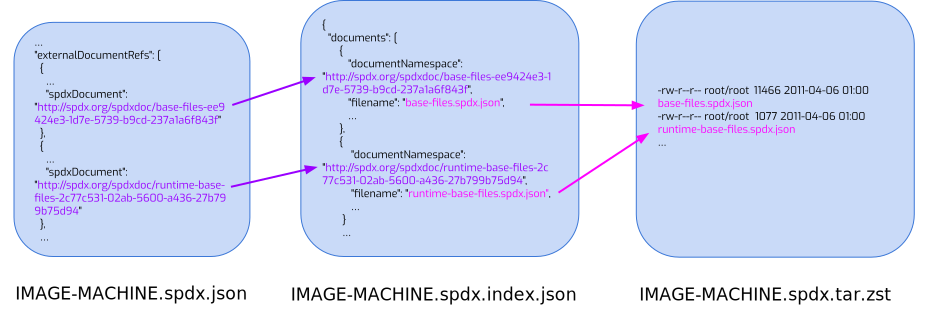
\includegraphics[width=\textwidth]{slides/yocto-licensing/spdx-sbom-output-details.pdf}
\end{frame}

\begin{frame}
  \frametitle{Further resources about SPDX SBoM}
    \begin{itemize}
       \item Yocto project documentation:\\
	     \url{https://docs.yoctoproject.org/dev/dev-manual/sbom.html}
       \item Joshua Watt: Automated SBoM generation with OpenEmbedded and the Yocto Project (FOSDEM 2023) \\
	     \url{https://youtu.be/Q5UQUM6zxVU}
       \item SPDX project homepage:\\
	     \url{https://spdx.dev}
    \end{itemize}
\end{frame}

